\section{Metodologías}

Una vez desarrollado el tema desde un punto de vista teórico, los pasos seguidos para realizar la parte práctica han sido los siguientes (Hernández, Fernández y Baptista, 2003):

\begin{enumerate} 
	\item Seleccionar el ambiente o lugar de estudio. Se ha elegido el sector hotelero y, en concreto, un hotel de la ciudad de Viena, Austria. 
	\item Elección de participantes o sujetos del estudio. La elección de los participantes ha sido aleatoria aunque tenían que cumplir el requisito de ser mayores de 18 años. 
	\item Inspección del ambiente o lugar de estudio. Las encuestas se realizaron en la recepción del hotel. 
	\item Trabajo de campo. Lectura y comprensión de los diferentes estadísticos para poder delimitar parámetros y estadísticos a aplicar. 
	\item Seleccionar el diseño de la investigación. Tras haber hecho la revisión de la literatura y  la obtención de los datos, se comenzó a aplicar los estadísticos elegidos y se obtuvieron los resultados. 

\end{enumerate}

Por lo tanto, el presente capítulo contiene las hipótesis del estudio de co-creación de valor, las variables seleccionadas para cada factor y los resultados del estudio estadístico. También, se discuten el diseño de investigación, la instrumentación y los métodos de análisis de datos.

\section{Características del cuestionario}

En este apartado, se describen las características del cuestionario utilizado. En el anexo \ref{anexo:7} se detalla el cuestionario y las instrucciones para llevarlo a cabo. Con dicho cuestionario se tratará de analizar la capacidad de co-creación de valor del hotel con respecto a la satisfacción, el bienestar, la participación, la fidelización de los clientes y los problemas que pueden darse a lo largo de la estancia. 

El cuestionario elegido, es de tipo mixto. Por un lado, hay preguntas dicotómicas en donde los individuos deben elegir entre las respuestas si y no. Y por otro lado, preguntas que son de tipo Likert, en las que se dan 5 opciones de respuesta al encuestado. Es una forma sencilla de calibrar opiniones específicas y da pie a crear escalas que pueden medir actitudes y valores más amplios. La escala va de uno 1 (muy insatisfecho) a 5 (muy satisfecho) con las afirmaciones propuestas (ver figura \ref{fig:escala}). Ambos grupos de preguntas serán tratados por separado y se elegirán diferentes métodos de evaluación para cada uno de ellos.

\begin{figure}[!h]
	\caption{Escala Likert aplicada en el cuestionario}
	\centering \includegraphics[width=150mm]{capitulos/graficos/escala} 
	\label{fig:escala} 
	
		\footnotesize
		Fuente: elaboración propia
\end{figure}

El huésped debe responder la opción que mejor se adapte a su realidad y con total sinceridad. Además, en cada pregunta, se da la posibilidad de aportar información extra referente a dicha cuestión. Con ello se pretende conocer más en profundidad las opiniones de los clientes, bien sean positivas o negativas para poder llevar a cabo mejoras estratégicas enfocadas al huésped.

\section{Características de la muestra}

Las 36 preguntas de la encuesta están dirigidas a huéspedes mayores de 18 años, que se han hospedado en el hotel más de una noche. El hotel está situado en capital de Austria, Viena. Hay que tener en cuenta que puede haber factores externos que alteren las respuestas de los clientes en el momento en el que se realiza el cuestionario (ver cuadro \ref{tab:respuestas}). Para controlar el efecto de estos factores, se ha realizado el test a clientes individuales en un lugar discreto y acogedor de la recepción, persiguiendo la máxima fiabilidad de los cuestionarios y solventando los problemas que pudieron surgir durante el test.

\begin{table}[h]
    \caption {Los factores que pueden afectar a las respuestas de los huéspedes}
	\label{tab:respuestas}
	\setlength\extrarowheight{5pt}
	
	\begin{tabular}{p{7cm} p{7.5cm}}
	\toprule
	Factores que pueden introducir cambios en los huéspedes                                           & Factores que pueden introducir cambios en las condiciones de administración                                                                             \\ 
\midrule
	Maduración.                 & La administradora del test.                           \\
	Aprendizaje e influencia general debida al medio social.       & El lugar elegido del hotel y su ambiente.                 \\
	Actividades anteriores a la administración del test.             & La hora y el día de la semana. \\
	Estado de salud de los huéspedes. & Sucesos no previstos durante la administración del test.                         \\ 
	\bottomrule
	\end{tabular}

	\center
	\footnotesize
	Fuente: elaboración propia
\end{table}


Se realizaron un total de 100 cuestionarios que fueron recogidos durante un período cinco meses entre diciembre del año 2014 y mayo de 2015. La figura \ref{fig:nacionalidades} muestra el porcentaje de nacionalidades que participaron en la encuesta. Además, la información demográfica general es la siguiente: de los 100 encuestados, el 45\% (45) eran hombres y el 55\% (55) eran mujeres. A efectos descriptivos, se considera una muestra lo suficientemente grande cuando $ n>30 $ por lo tanto, se ha considerado que la muestra es suficiente para llevar a cabo el estudio estadístico a un nivel de seguridad del 95\% (Jimenez, 1983).

\begin{figure}[!h]
	\caption{Nacionalidades de los encuestados}
	\centering 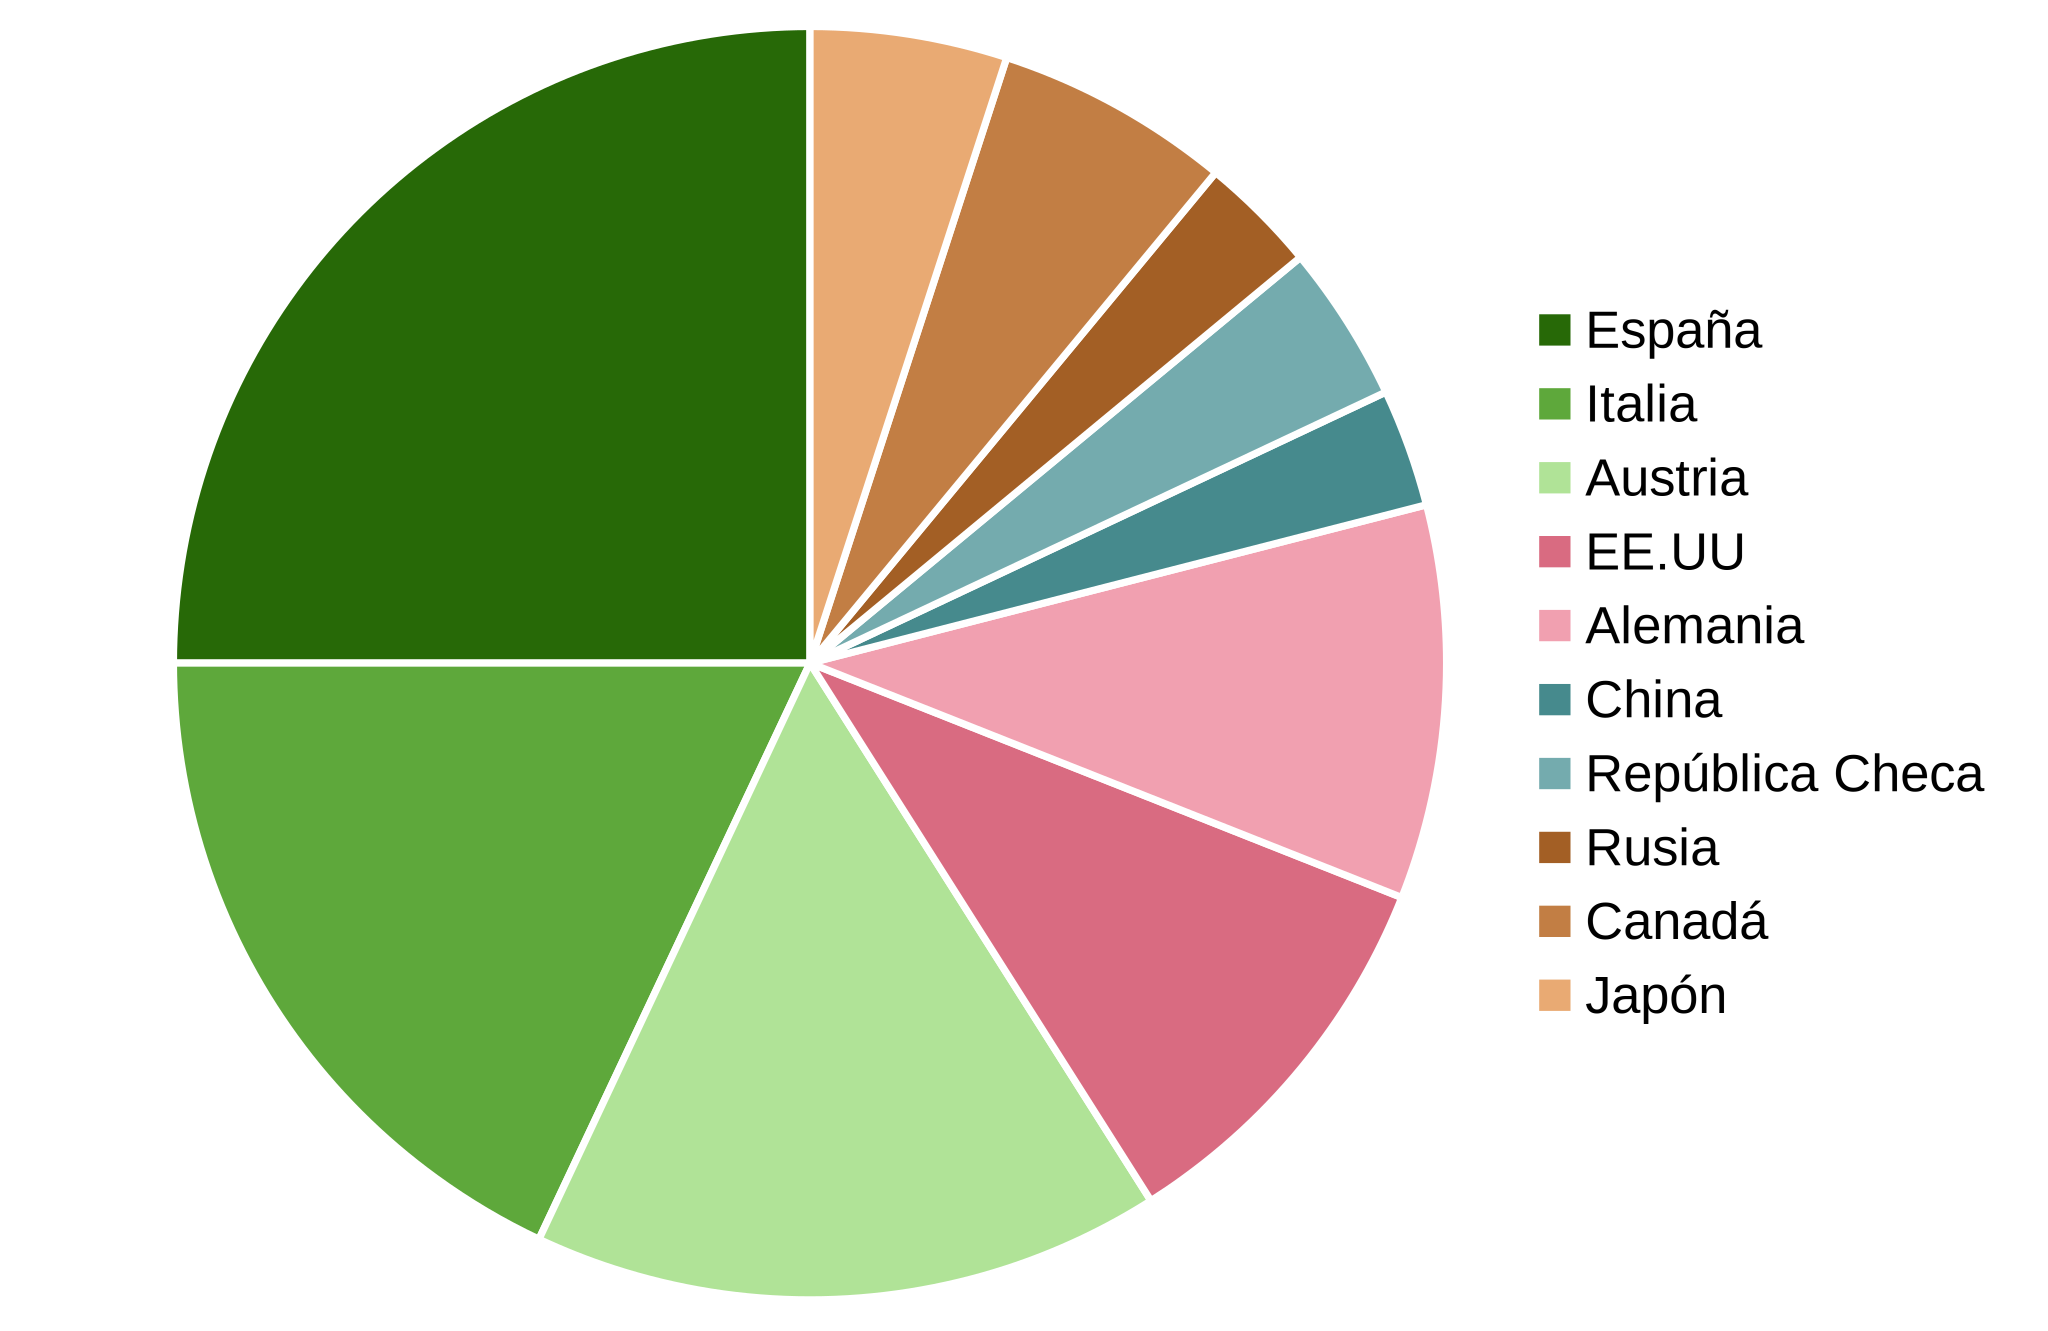
\includegraphics[width=120mm]{capitulos/graficos/nacionalidades} 
	\label{fig:nacionalidades} 
	
		\footnotesize
		Fuente: elaboración propia
\end{figure}

\section{Definición de los factores}

Para poder llevar a cabo este estudio, es necesario definir los factores que se quieren analizar y explicar el porqué de su elección. Los factores elegidos son apoyados por diversos autores que recoge Frances (2013), autora que se va a tener en cuenta en este presente epígrafe.

\subsection{Co-creación}

Frances (2013) indica que algunos investigadores (Cova et al., 2011, y Arvidsson, 2008) creen que fundamental la voluntad del cliente a la hora de trabajar y de participar con la empresa. Sin esta interacción la co-creación de valor no es posible. Sin embargo, si la empresa propone un proceso de co-creación de valor con el cliente, hay que tener en cuenta que los consumidores han de tomar la decisión de si desean o no co-crear valor con el hotel. Para Frances (2013), la co-creación se basa en la unión de dos partes, en este caso serían el huésped y el hotel. Por lo tanto, en este estudio se pretende medir cómo afecta la disposición de los huéspedes a la hora de co-crear valor trabajando codo con codo con el hotel, compartiendo sus ideas, problemas y sentimientos de bienestar, expresando sus opiniones bien sean satisfactorias o insatisfactorias, midiendo el grado de fidelización y de participación de los clientes. Para ello, el hotel ha de contar con un personal adecuado que sepa transmitir los valores de la cadena hotelera, también ha de estar abierto a escuchar e incorporar las ideas de cada huésped, y además ha de ser capaz de facilitar la co-creación y proporcionar un ambiente que propicie la unión de ambas partes para que los clientes sientan que sus opiniones son escuchadas y valoradas, y fomentar que el cliente se sienta valorado y mimado por el hotel. Esta continua transformación es vital para que surja la co-creación de valor (Frances, 2013). 

\subsection{Satisfacción}

Según Frances (2013), la satisfacción puede confundirse con el bienestar del cliente. Si la satisfacción aumenta, el bienestar también debería de hacerlo. Pero en el presente trabajo se va a considerar como satisfacción el momento en el que el cliente evalúe la relación de experiencias que ha establecido con el hotel teniendo en cuenta también su nivel de vida. Por lo tanto, este factor indicará que si el cliente está lo suficientemente satisfecho con lo que el hotel le ha proporcionado a lo largo de su estancia, entonces aumentará la posibilidad de que el consumidor vuelva. También, se podrá evaluar si el cliente cree que está acorde lo que se le ha ofrecido con lo que ha pagado por ello. Además, podrá utilizar el boca a boca para expresar su satisfacción a a través de las redes sociales o personalmente acerca del hotel.

\subsection{Bienestar}

Este factor tiene en cuenta aspectos como la valoración del medio ambiente que rodea al hotel y el trato percibido por el cliente por parte del personal (Frances, 2013). Según Frances (2013), los efectos económicos como los ingresos, el empleo, el coste de vida, los precios de bienes y servicios, y los impuestos, afecta al bienestar percibido por un huésped. Se puede dar el caso de que algunos clientes puedan sentirse limitados a participar en estos procesos de co-creación porque éste no disponga de los recursos personales necesarios para contribuir al intercambio de experiencias, y por lo tanto se ve afectado su bienestar. Por otro lado, los efectos ambientales tales como la contaminación o el tráfico, también pueden influir en el bienestar del huésped. No se trata de una variable fundamental dentro del proceso de co-creación de valor, pero si que hay que tener en cuenta que si un cliente busca tranquilidad y se le ofrece una habitación con orientación a una calle muy transitada y con tráfico pesado o con zonas contaminadas, esto daría lugar a una negativa experiencia de alojamiento y un nivel de bienestar muy bajo. Este efecto podría provocar que el cliente no vuelva al hotel y viceversa en caso contrario. Por lo tanto, con el fin de mejorar el bienestar del cliente, las interacciones entre el personal del hotel y los huéspedes en los procesos de co-creación han de ser positivas.

\subsection{Participación}

Según indica Frances (2013), los autores Grissemann y Stokurger-Sauer (2012) y Lee (2012) demostraron que en la co-creación de valor influye el grado de participación que el cliente tiene. En el presente estudio, se va a medir a través de las implicaciones que los clientes tienen con otros huéspedes; analizando si participan activamente en ONGs cercanas al hotel; o teniendo en cuenta si los huéspedes administran los recursos naturales de forma responsable; analizando si contribuye al desarrollo económico tanto de la ciudad de Viena como de este hotel en concreto y por último, si está dispuesto a publicar su opinión en Tripadvisor que es la Web líder mundial de opiniones de hoteles.

\subsection{Problemas}

En el presente trabajo se quiere evaluar si los problemas afectan a los procesos de co-creación y para ello se va tener en cuenta si a los huéspedes les surgen un gran número de problemas y al mismo tiempo si estos problemas los reportan al personal del hotel y este a su vez los resuelve eficazmente. Se va a suponer que si existe gran cantidad de problemas, los procesos de co-creación no se desarrollarán favorablemente y viceversa.

\subsection{Fidelización}

Se trata de efectos sociales, donde se tiene en cuenta la calidad de las interacciones entre los clientes y los empleados y las posteriores relaciones resultantes. Se espera que los efectos sociales de esta fidelización estén directamente relacionados con la co-creación. Para ello, se requiere mucha interacción duradera en el tiempo entre el huésped y el hotel para crear una relación de fidelización. Esto se puede conseguir si un cliente es capaz de trabajar de manera efectiva junto con la empresa hotelera, propiciando un desarrollo de la relación mucho más fuerte y que tiene un efecto positivo en la fidelización del cliente con la cadena hotelera. En cambio, si la relación no tiene éxito y el huésped siente que el hotel no le proporciona lo que desea, o siente que no tiene la oportunidad de participar en el proceso de co-creación de valor, entonces la relación de fidelización no surgirá (Frances, 2013).

\section{Formulación de las hipótesis}

Una vez descritos los factores que se quieren estudiar, se ha de recordar que principal objetivo del estudio es el de medir el grado de relación entre la co-creación de valor por parte de los clientes y la satisfacción y el bienestar, además, se quiere determinar la relación sobre la implicación que los clientes asumen en el programa de fidelización, la participación y cómo afectan los problemas que les surgen a los huéspedes con respecto a la co-creación de valor con el hotel. Por ello, se van a plantear las siguientes  hipótesis (ver figura \ref{fig:hipotesis}):

\begin{itemize}
\item H1: Existe una relación directa entre la co-creación de valor y la satisfacción del cliente en el hotel.

\item H2: Existe una relación directa entre la co-creación de valor y el bienestar del cliente en el hotel.

\item H3: Existe una relación directa entre la co-creación de valor y la participación del cliente con el hotel.

\item H4: Existe una relación directa entre la co-creación de valor y los problemas que le surgen a los huéspedes en el hotel.

\item H5: Existe una relación directa entre la co-creación de valor y la fidelización de los clientes.
\end{itemize}

\begin{figure}[!h]
	\caption{Hipótesis}
	\centering 
\includegraphics[width=150mm]{capitulos/graficos/hipotesis} 
	\label{fig:hipotesis} 
	
		\footnotesize
		Fuente: elaboración propia
\end{figure}

Estas hipótesis se pueden relacionar con las teorías sobre la co-creación de valor desarrolladas en el capítulo \ref{section:cocreacion} del presente trabajo. En primer lugar, la integración de recursos que recoge la lógica dominante del servicio se puede relacionar con la hipótesis H3 que evalúa si hay una relación directa entre la co-creación de valor y la participación del huésped. Lo hace a través de cuestiones por las que se integran recursos en el proceso co-creativo, por ejemplo, con la participación en ONGs, la administración de los recursos naturales, el desarrollo económico por parte del huésped, etc. En segundo lugar, se encuentra la interacción que rompe con los procesos de producción de productos para desarrollar uno propio para los servicios. Eigler y Langeard desarrollan la teoría de la servucción y la escuela nórdica de Grönroos la lógica del servicio. Las hipótesis H4 y H5, se corresponde con el análisis de la relación directa entre la co-creación de valor y los problemas que le surgen al cliente y la fidelización de éste respectivamente. Son los factores que requieren que el personal del hotel y el huésped interactúen entre sí. Y por último, las hipótesis H1 y H2, evalúan la relación que tiene la co-creación de valor con la satisfacción y con el bienestar, encajan con la teoría de Prahalad y Ramaswamy que defienden las relaciones personalizadas entre la empresa y el cliente para que éste último pueda interaccionar con el entorno empresarial y cree experiencias personales de co-creación de valor tanto para la empresa como para sí mismo. 

\section{Análisis de datos}

En esta sección del capítulo 2, se resumirán los pasos a seguir en el análisis de datos. Tras el proceso de recogida de datos, éstos se han procesado y ordenado con el fin de llevar acabo un análisis fiable. Para ello, se ha elegido el programa informático IBM SPSS Statistics 23. Se trata del Software estadístico líder mundial utilizado para resolver problemas empresariales y de investigación por medio de análisis ad-hoc, pruebas de hipótesis y análisis predictivo (ibm.com, 2015).

Como el cuestionario es de tipo mixto, se van a realizar dos estudios preliminares diferentes para determinar qué variables se asocian a los diferentes factores a estudiar. Ambos análisis, se van a dividir en dos estudios a su vez. En el primero de ellos, se va a realizar un análisis factorial y posteriormente un contraste de hipótesis a través de la varianza denominado ANOVA. Para el estudio de las variables dicotómicas el análisis factorial es subjetivo y el investigador decidirá las variables que han de incorporarse a cada factor (Montoya, 2007; Mora, 2010), ya que el cuestionario dicotómico fue elaborado con esta intención. En el cuadro \ref{tab:criterios}, se pueden apreciar los cálculos que se van a llevar a cabo a lo largo del análisis y los límites que propone la literatura.

\begin{table}[h]
    \caption {Criterios utilizados en el estudio estadístico}
	\label{tab:criterios}
	\setlength\extrarowheight{5pt}
	
	\begin{tabular}{p{2.1cm} p{3.5cm} p{4.2cm} p{4.1cm}}
	\toprule
	Análisis factorial	& Cargas factoriales	& $ > 0,4 $	& Everitt y Hothorn, (2011)	\\
						& Autovalores			& $ > 1 $		& Everitt y Hothorn, (2011)	\\
						& Alfa de Cronbach		& $ > 0,7 $	& Everitt y Hothorn, (2011)	\\
						& Varianza acumulada	& $ > 0,65 $	& Everitt y Hothorn, (2011)	\\
						& Test de esfericidad de Bartlett & $ p < 0.05 $ & Blasco, 2014; Mora, 2012; Thorndike, 1989; Montoya, 2007	\\
						& Kaiser Meyer Olkin	& \pbox{4.2cm}{
						$ KMO < 0,5 $: no existe correlación. \\
						$ 0,5 < KMO < 0,6 $: nivel de correlación medio. \\
						$ KMO > 0,7 $: alta correlación. \\
						} & Blasco, 2014; Mora, 2012; Thorndike, 1989; Montoya, 2007	\\
	\midrule
	Contraste de hipótesis	& ANOVA				& $ p < 0.05 $	& Rolan, 2014 \\
	\bottomrule
	\end{tabular}
	
	\center
	\footnotesize
	Fuente: elaboración propia
\end{table}


\subsection{Estudio 1}

\subsubsection{Análisis factorial}

El análisis factorial tuvo sus orígenes a comienzos del siglo XX y es conocido como una técnica estadística de interdependencia que se caracteriza por su versatilidad. Esta técnica consiste en analizar un grupo de variables que se analizan al mismo tiempo y en conjunto (Menendez y Rondón, 2012). Uno de los objetivos de este análisis es tratar de definir grupos de variables que a partir de ahora se les va a denominar factores, y que deben de estar altamente correlacionados entre sí. Otros dos objetivos son la reducción de la complejidad en cuanto al número de variables a utilizar en el estudio y eliminar variables redundantes o que aporten poca información. Por lo tanto, va a permitir explicar el fenómeno de la co-creación de valor deforma más minuciosa. Y por último, va a ayudar a identificar problemas de multicolinealidad evaluando si las variables altamente correlacionadas pueden afectar a la construcción de los modelos de regresión o de análisis multivariantes (Montoya, 2007).

Los cálculos se van a realizar en SPSS a partir de la \emph{matriz original de datos} \footnote{Se corresponde a la matriz que contiene las 36 variables bajo estudio con las correspondientes 100 observaciones por variable.} creada en un documento Excel. En el anexo \ref{anexo:8} se pueden encontrar todos los resultados de este análisis. En primer lugar, SPSS calculará la \emph{matriz de correlaciones} de las variables medidas en escala Likert, que mide y muestra la interdependencia entre cada pareja de variables y todas al mismo tiempo (Peña, 2002; Lemos, Vallejo y Sandoval, 2002; Montoya, 2007). Al mismo tiempo, calculará el determinante de esta matriz de correlaciones cuyo valor ha sido $ D = 4,85E-009 $, el cual se considera muy bueno porque significa que hay variables que poseen intecorrelaciones muy altas y se puede continuar con el análisis (Lemos, Vallejo y Sandoval, 2002; Montoya, 2007).

Por otro lado, se calcula el índice de \emph{Kaiser Meyer Olkin} (KMO) cuyo valor ha sido de 0,611 que indica que existe un nivel de correlación medio una vez que se han descontado los efectos lineales de otras variables (Blasco, 2014; Mora, 2012; Thorndike, 1989: Montoya, 2007). Además, la \emph{prueba de esfericidad de Bartlett} ha resultado tener una fiabilidad de $ p = 0,000 $, por lo tanto, el nivel de significación es menor a p < 0.05, lo que significa que se rechaza la hipótesis nula y se continúa con el análisis factorial (Blasco, 2014; Mora, 2012; Jackson, 1993; Bossé et. al. 1999; Montoya, 2007).

En tercer lugar, se calcula la \emph{matriz anti-imagen} donde se ha observado que no existen a penas coeficientes cero y por lo tanto se continua el análisis (Montoya, 2007).

El siguiente paso es comprobar la \emph{varianza total explicada} que es la que agrupa a las variables a partir del total de la variabilidad del número de variables. El límite que establece la comunidad para aceptar la fiabilidad del estudio y continuarlo, es que la varianza acumulada debe de ser mayor a 65\% y en el caso a estudiar, dicha varianza adquiere un valor de 66,533848\% (Damey, Andams y Freites, 1992).

La función del \emph{gráfico de sedimentación} es localizar visualmente un codo o punto de inflexión,que puede ser definido como el punto donde los valores propios forman una tendencia lineal descendente (Reise, Waller y Comrey, 2000).

A continuación, se obtendrá la \emph{matriz de componentes} con la extracción inicial y una segunda matriz con la peculiaridad de que es la matriz de componentes rotada por VARIMAX. Esta rotación, se realiza con la finalidad de lograr una solución que facilite la interpretación (Montoya, 2007). La rotación Varimax es uno de los métodos más utilizados en la actualidad para la formación de los componentes cuyos ítems serán aceptados si superan la barrera del 0,4 (Martínez, 2008; Montoya, 2007). Las variables finales asignadas a cada factor son las mostradas en el cuadro \ref{tab:variablesFactores1}. Y se corresponde con la solución que ha proporcionado SPSS a través del cuadro de resultados denominada \emph{matriz de factores rotados}, donde los coeficientes de esta matriz indican cuánto explica cada variable los factores surgidos y por lo tanto los encasilla en un factor u otro teniendo en cuenta dos aspectos: 1) el coeficiente ha de ser mayor a 0,40 y, 2) el factor elegido ha de ser superior en 0,10 al segundo mejor factor (universidad de Monterrey, 2012). La denominación de los factores encontrados, McDaniel et al. (1999) señalan que es algo subjetivo y se requiere de una combinación de intuición y conocimiento por parte del investigador sobre las variables.

\begin{table}[h]
    \caption {Variables de los factores del estudio 1}
	\label{tab:variablesFactores1}
	\setlength\extrarowheight{5pt}
	
	\begin{tabular}{p{11.8cm} p{2.9cm}}
	\toprule
	¿Recomendará este hotel? & \\
	¿Volverá a este hotel? & \\
	¿Está satisfecho con baño de la habitación? &  \\
	¿Está satisfecho con las amenidades del baño y los productos de aseo que el hotel el proporcionó? & Satisfacción \\
	¿Cómo evalúa la relación calidad – precio global? & \\
	¿Está satisfecho con el servicio de desayunos? & \\
	\midrule
	¿Cómo fue su experiencia global en el hotel? & \\
	¿Cómo fue su experiencia global con la habitación? & \\
	¿Qué le pareció la atmósfera del hotel (música, aroma, iluminación, decoración, mobiliario)? & \\
	¿Qué le pareció la cama? & Bienestar \\
	¿Cómo fue su experiencia durante el Check in? & \\
	¿Cómo evalúa los servicios de Internet y WiFi en el hotel? & \\
	¿Cómo evalúa la atención al huésped en general en el hotel? & \\
	¿Su reserva antes de llegar al hotel fue gestionada eficientemente? & \\
	\midrule
	¿Cómo ha sido la actitud y proactividad de los empleados durante su estancia en el hotel? & \\
	¿Cómo ha sido el trato de los empleados a lo largo del check out? & Co-creación \\
	¿Sintió que le mimamos durante su estancia? & \\
	¿Le parece adecuado el plan de fidelización que propone el hotel? & \\

	\bottomrule
	\end{tabular}
	
	\center
	\footnotesize
	Fuente: elaboración propia
\end{table}


\newpage

A continuación, en el cuadro \ref{tab:afe} se van a resumir algunos de los resultados obtenidos en el análisis factorial y por los cuales se ratifica que estos son los factores a analizar en el contraste de hipótesis.

\begin{table}[h]
    \caption {Análisis exploratorios de fiabilidad y dimensionalidad}
	\label{tab:afe}
	\setlength\extrarowheight{5pt}
	
	\begin{tabular}{p{1.9cm} p{1.9cm} p{1.9cm} p{1.9cm} p{1.9cm} p{1.9cm} p{1.7cm}}
	\toprule
	Factor	& Coeficiente menor de cargas factoriales	& Autovalores & Alfa de Cronbach & Varianza explicada & Test de esfericidad de Bartlett & KMO \\
	\midrule
	Co-creación	 & 0,7	& 2,511	& 0,783	& 28,106 & 0,000 & 0,665 \\
	Satisfacción & 0,45	& 3,465	& 0,837	& 22,524 & 0,000 & 0,812 \\
	Bienestar	 & 0,57	& 3,886	& 0,835	& 28,106 & 0,000 & 0,814 \\
	\bottomrule
	\end{tabular}
	
	\center
	\footnotesize
	Fuente: elaboración propia
\end{table}


\newpage


\subsubsection{Contraste de hipótesis}

Una vez que se han verificado los factores a través del análisis factorial, a continuación se van a testar las dos primeras hipótesis propuestas con el método ANOVA. Este método, viene de la terminología inglesa \emph{analysis of variance}, cuya traducción al castellano es análisis de la varianza.

El análisis ANOVA permite relacionar los factores satisfacción y bienestar con el factor de co-creación de valor de una forma directa. De esta forma, se podrán contrastar las hipótesis nulas planteadas al comienzo del capítulo. Los cálculos llevados a cabo con SPSS se pueden apreciar en el anexo \ref{anexo:9}.
La interpretación de los resultados relevantes mostrados en el cuadro \ref{tab:anovaSB}, determinan la relación existente entre la satisfacción y el bienestar con la co-creación de valor. En primer lugar, se va a analizar la satisfacción, donde su nivel crítico asociado al estadístico es $ F_{4,929} $ es $ p = 0,04 $. El criterio establece que $ p = 0,000 < 0,05 $, por lo tanto, este resultado indica que el modelo explica una parte significativa de la variación observada en el factor co-creación. Como consecuencia, se puede confirmar la hipótesis 1 que afirma que existe una relación directa entre la satisfacción y la co-creación de valor. En cambio para el factor bienestar, el nivel crítico asociado al estadístico $ F_{2,111} $ es $ p = 0,107 $ que es mayor que 0,05, lo que hace que se la hipótesis 2 se rechace y se establezca que no existe una relación directa entre el bienestar y la co-creación de valor.

\begin{table}[h]
    \caption {Resultados ANOVA de la satisfacción y el bienestar con respecto a la co-creación de valor}
	\label{tab:anovaSB}
	\setlength\extrarowheight{5pt}
	
	\begin{tabular}{p{4.0cm} p{4.6cm} p{3.1cm} p{2.1cm}}
	\toprule
	Origen	& Media cuadrática	& F & Sig. \\
	\midrule
	Satisfacción & 1,474	& 4,929	& 0,004 \\
	Bienestar	 & 1,199	& 2,111	& 0,107 \\
	\bottomrule
	\end{tabular}
	
	\center
	\footnotesize
	Fuente: elaboración propia
\end{table}


\subsection{Estudio 2}

\subsubsection{Análisis factorial}

En el caso de las cuestiones dicotómicas, a la hora de realizar el cuestionario se establecieron tres grupos y se ha creído conveniente que esos grupos de variables sean los factores finales para el análisis (Montoya, 2007; Mora, 2010).

Para comprobar si los factores son fiables se ha calculado el coeficiente \emph{alfa de Cronbach}, que fue propuesto por primera vez en 1951 por Lee Cronbach. Se trata de un estadístico que estima la confiabilidad de una prueba a partir de la suma de varias mediciones (Thorndike, 1989,1996; Muñiz, 1996). A través del cálculo de los alfas de Cronbach, se puede valorar la fiabilidad de las escalas de medida elegidas y evaluar si los huéspedes han contestado de forma coherente a este tipo de preguntas dicotómicas. Además, se han contrastado los resultado con el coeficiente de Kuder Richardson (KR-20), ya que es análisis que más utilizado para medir variables dicótomicas, los resultados han sido idénticos (ver anexo \ref{anexo:10}). Por lo tanto, los factores que se han delimitado para las cuestiones dicotómicas son: participación, problemas y fidelización; quedando las variables enumeradas tal y como aparecen en el cuadro \ref{tab:variablesFactores2}). 

\begin{table}[h]
    \caption {Variables de los factores del estudio 2}
	\label{tab:variablesFactores2}
	\setlength\extrarowheight{5pt}
	
	\begin{tabular}{p{11.8cm} p{2.9cm}}
	\toprule
	¿Le gustaría enviar su opinión a Tripadvisor a través de esta encuesta?	& \\
	¿Proporciona usted productos y servicios sostenibles a otros huéspedes?	& \\
	¿Promueve la oferta cultural de la ciudad de Viena?	& Participación \\
	¿Apoya las actividades de las ONGs y otras organizaciones locales?	& \\
	¿Administra los recursos naturales de una forma responsable (agua, energía, desperdicios)?	& \\
	¿Contribuye al desarrollo económico de este hotel con su estancia?	& \\
	\midrule
	¿Tuvo algún problema?	& Problemas \\
	¿Reportó ese problema?	& \\
	\midrule
	¿Es miembro del programa de fidelidad? & \\
	¿Durante su estancia, ¿le informaron sobre los beneficios del programa de fidelidad? & Fidelización \\
	¿Se hizo miembro del programa de fidelidad durante la última estancia? & \\
	\bottomrule
	\end{tabular}
	
	\center
	\footnotesize
	Fuente: elaboración propia
\end{table}


\subsubsection{Contraste de hipótesis}

Una vez se han delimitado los factores, a continuación se va a proceder a testar las tres últimas hipótesis propuestas con el método ANOVA como ya se ha realizado en el estudio 1. Al tratarse de variables categóricas, se ha utilizado otra de las opciones que propone SPSS. Se pueden comprobar los resultados obtenidos en el anexo \ref{anexo:11}.

La interpretación de los resultados relevantes mostrados en el cuadro \ref{tab:anovaPPF}, determinan la relación existente entre la participación, los problemas y la fidelización con la co-creación de valor. En primer lugar, se va a analizar la participación, donde su nivel crítico asociado al estadístico es $ F_{3,686} $ es $ p = 0,04 $. El criterio establece que $ p = 0,000 < 0,05 $, por lo tanto, este resultado indica que el modelo explica una parte significativa de la variación observada en el factor co-creación. Como consecuencia, se puede ratificar la hipótesis 3 que afirma que existe una relación directa entre la participación y la co-creación de valor. En cambio para el factor problemas, el nivel crítico asociado al estadístico $ F_{0,03} $ es $ p = 0,959 $ que es mucho mayor que 0,05, lo que hace que la hipótesis 4 se rechace y se establezca que no existe una relación directa entre el los problemas surgidos al huésped en el hotel y la co-creación de valor. Y por último, el factor fidelización tiene un nivel crítico asociado al estadístico de $ F_{3,463} $ es $ p = 0,023 $, por lo tanto, este resultado indica que el modelo explica una parte significativa de la variación observada en el factor co-creación. Como consecuencia, se puede ratificar la hipótesis 5 que afirma que existe una relación directa entre la fidelización del huésped y la co-creación de valor.

\begin{table}[h]
    \caption {Resultados ANOVA de la participación, los problemas y la fidelización con respecto a la co-creación de valor}
	\label{tab:anovaPPF}
	\setlength\extrarowheight{5pt}
	
	\begin{tabular}{p{2.9cm} p{2.9cm} p{2.9cm} p{2.9cm}}
	\toprule
	Origen	& Media cuadrática	& F & Sig. \\
	\midrule
	Participación	& 17,174	& 3,686	& 0,04 \\
	Problemas	 	& 0,03		& 0,03	& 0,959 \\
	Fidelización	& 9,069		& 3,463	& 0,023 \\
	\bottomrule
	\end{tabular}
	
	\center
	\footnotesize
	Fuente: elaboración propia
\end{table}


A continuación, se va a presentar el cuadro \ref{tab:hipotesis} en el que se puede apreciar la solución final de la parte empírica de este trabajo y por lo tanto la solución final al objetivo principal de este proyecto que es determinar las relaciones de diferentes factores con la co-creación de valor. Además, se va a proceder a realizar una comparativa entre los resultados obtenidos y la visión que el hotel tiene acerca de estas relaciones gracias a la entrevista realizada a un directivo del hotel. En el anexo \ref{anexo:12} se puede encontrar las preguntas realizadas en la entrevista.

\begin{table}[h]
    \caption {Solución del contraste de hipótesis}
	\label{tab:hipotesis}
	\setlength\extrarowheight{5pt}
	
	\begin{tabular}{p{2.1cm} p{9.7cm} p{2.3cm}}
	\toprule
	Número	& Hipótesis	& Se acepta / se rechaza \\
	\midrule
	H1 & Existe una relación directa entre la co-creación de valor y la satisfacción del huésped en el hotel.	& Aceptada \\
	H2 & Existe una relación directa entre la co-creación de valor y el bienestar del huésped en el hotel.	& Rechazada \\
	H3 & Existe una relación directa entre la co-creación de valor y la participación del huésped con el hotel.	& Aceptada \\
	H4 & Existe una relación directa entre la co-creación de valor y los problemas que le surgen a los huéspedes en el hotel.	& Rechazada \\
	H5 & Existe una relación directa entre la co-creación de valor y la fidelización de los huéspedes.	& Aceptada \\	
	\bottomrule
	\end{tabular}
	
	\center
	\footnotesize
	Fuente: elaboración propia
\end{table}


Tal como se puede apreciar en el cuadro \ref{tab:hipotesis}, el bienestar, la participación y la fidelización de los huéspedes tienen una relación directa con la co-creación de valor; y por el contrario, el bienestar y el surgimiento de problemas en el hotel no tienen una relación directa con la co-creación de valor. En el anexo \ref{anexo:13}, se explica la relación entre el hotel y los clientes, desde el punto de vista del director de hotel. A continuación, teniendo en cuenta estas explicaciones, se va a dar sentido a los resultados de las hipótesis formuladas en el presente capítulo teniendo en cuenta el punto de vista del director del hotel.

Según el estudio realizado, existe una relación directa entre la co-creación de valor y la satisfacción del huésped. Señala la importancia de la variable relación calidad – precio en la percepción de satisfacción del cliente. Además, para el director del hotel, que un cliente se vaya satisfecho garantiza dos cosas: que volverá y que hablará del hotel a sus familiares y amigos, produciendose así la mejor y la más económica de todas las publicidades de las que disponen en la cadena. Además, afirma que cuando se da este caso, la reputación del establecimiento aumenta considerablemente y como consecuencia se generan ingresos. Como bien se ha tratado a lo largo del trabajo, no todos los clientes son iguales, y el director del hotel lo ratifica. Existen multitud de perfiles de clientes, tantos como motivos de viajes, nacionalidades, etc. Pero también destaca que no siempre tienen razón y no siempre se les puede hacer caso en todo lo que proponen. Por ejemplo, realizar una reforma en el bar para convertirlo en estilo chill out se puede considerar como una muy buena idea y que revalorizaría al hotel, pero otro cliente puede opinar lo contrario. Además, hay que tener en cuenta que el hotel puede no disponer de los medios y de la financiación para llevarlo a cabo. También le surge la preocupación del boca a boca, ya que si los clientes han finalizado la estancia con un grado alto de insatisfacción harán uso de Internet y de las redes sociales para divulgar su frustración. Por lo tanto, se puede decir que si el cliente finaliza satisfecho, tanto el hotel como el huésped habrán conseguido co-crear valor conjuntamente.

En segundo lugar, el estudio establece que no existe una relación directa entre la co-creación de valor y el bienestar del huésped. Esta cuestión entra en discordancia con la visión que el director tiene sobre este punto. Éste, asume que si el cliente no ha obtenido el bienestar esperado se debe a que el hotel no ha sabido adaptarse a las necesidades del huésped. El objetivo que tiene el hotel con respecto a este factor, es dar cabida a las expectativas del cliente y superarlas en todo momento. Para hacer que el huésped desarrolle su bienestar, en cada hotel existe una persona que ostenta el cargo de “Guest experience”, o traducido al castellano “jefe de calidad”. Esta persona es la encargada de atender a los clientes y de hacerles más agradable su estancia, pero también es la responsable de inculcar los valores de la cadena a los trabajadores.

El primer paso en la formación del personal del hotel, es una reunión donde se les facilita un manual de conducta y otros aspectos a tratar. Por ejemplo, la fraseología que los empleados han de utilizar con el cliente. Hay departamentos que al tener más contacto con el cliente, se ha de prestar especial énfasis en esta parte. Además, en dicha reunión se emplean vídeos desarrollados por el departamento de recursos humanos para poner ejemplos de cómo se ha de actuar en un determinado momento y circunstancia. También, hay que tener en cuenta que a mayor responsabilidad en el cargo que se ostente dentro de la empresa, mayor conocimiento se exige sobre el cliente. Por ello, este aspecto es muy importante para el hotel, y se puede decir que se discrepa con los resultados obtenidos en el estudio.

En cuanto a la relación directa existente, según los resultados del estudio, entre la co-creación de valor y la participación del cliente, el director del hotel destaca la importancia de que el cliente se involucre de una forma muy activa, bien sea por iniciativa propia o del hotel. Esta participación genera reputación y riqueza, y la generación de riqueza es fundamental para la empresa. Sin dinero y sin retorno del cliente, no hay beneficio y si no hay beneficio el negocio no es rentable. Además, la participación del huésped también puede generar publicidad a través del boca a boca a parte de riqueza. Por lo tanto, queda demostrado que la co-creación de valor y la participación del cliente con el hotel van de la mano.

Por otro lado, el estudio indica que no existe una relación directa entre la co-creación de valor y los problemas que le puede surgir al huésped, se trata de un resultado totalmente acorde con lo esperado y con lo que el director del hotel ha expresado. La forma de interactuar en el momento en el que surgen problemas es mediante la comunicación directa entre cliente y personal del hotel. Otro modo, es mediante las encuestas de calidad donde queda registrada la opinión del cliente, y es en ese momento en el que la cadena hotelera acepta que existe un problema y puede o no otorgar los medios físicos o monetarios para poder atajar los problemas. Pero la realidad, según indica el director con total sinceridad, es que muchos de los problemas se almacenan y no se solventan en un largo periodo de tiempo, ya que siempre suelen existir otras prioridades.

Y por último, la relación directa que hay entre la co-creación de valor y la fidelización del huésped es un punto muy destacado por el director del hotel. Este programa de fidelización que propone la cadena hotelera es idéntico en cada hotel independientemente de su localización. Esto supone, que el cliente va a recibir el mismo trato y las mismas ventajas en un hotel de una ciudad u otra. Para que esta fidelización se produzca, la compañía tiene que proporcionar al cliente unas ventajas y un trato superior a los competidores. Una vez que un cliente que pertenece al plan de fidelización y abandona un hotel, la cadena se pone en contacto con él para que éste pueda valorar su estancia. Todas las sugerencias se archivan para una futura ocasión aunque el servicio post venta como tal no exista. Para solventar este problema, la cadena está desarrollando una nueva base de datos con la que pretenden personalizar las experiencias de los huéspedes fidelizados facilitándoles y sugiriéndoles opciones de viaje adecuadas a sus gustos. El mayor fracaso que puede sufrir el hotel es no cumplir las expectativas de un cliente por un motivo u otro. Por ello, que se de una relación de fidelización, hace que la co-creación de valor surja de una forma espontánea. 

Se puede concluir el presente estudio, afirmando que son resultados esperados a excepción del bienestar, ya que podría darse el caso de que un cliente que no haya estado lo suficientemente satisfecho en cuanto al bienestar subjetivo que ha percibido, participase en los procesos de co-creación. Por otro lado, el surgimiento de los problemas va a propiciar que el cliente no participe activamente en estos procesos de co-creación de valor. Y por último, es razonable que un cliente satisfecho, participativo y fidelizado con el hotel si que forme parte de los procesos co-creativos de valor.
